\chapter{Harmonogram Realizacji Projektu}
\label{cha:harmonogramRealizacjiProjektu}

Najtrudniejszym było zapoznać się z nowymi technologiami, takimi jak JavaFX i Hibernate, oraz LaTeX, ponieważ wcześniej pracowałem głównie z JDBC i Swing. Jednakże, dzięki książkom, tutorialom na YouTube, stackoverflow, udało mi się szybko opanować podstawy tych technologii.

Odpowiednio do wymagań, stworzyłem diagram Gantta, który widziano poniżej:

\begin{figure}[h!]
    \centering
    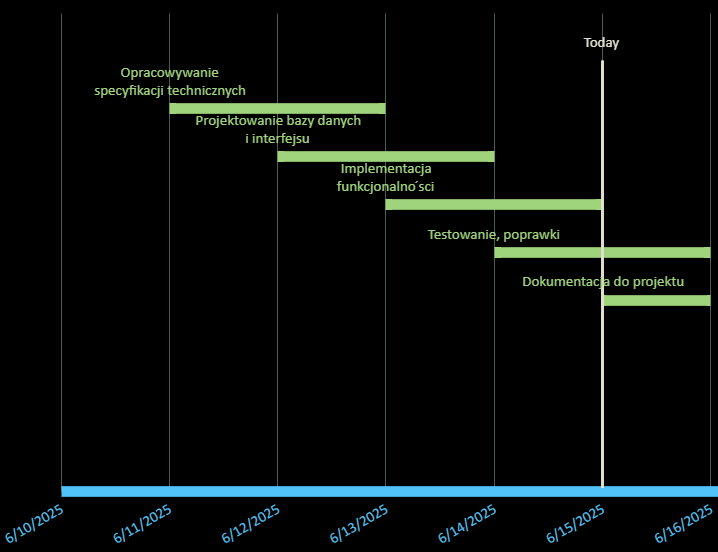
\includegraphics[width=0.8\textwidth]{figures/Gantt.png}
    \caption{Diagram Gantta \label{fig2}}
\end{figure}

\subsection{Repozytorium}

Kod źródłowy projektu jest dostępny w repozytorium GitHub pod adresem: \url{https://github.com/kayor1x/ProjectJava1rok}

